\subsubsection{x86: 3 argomenti}
% to be sync: \subsubsection{x86: 3 integer arguments}

\myparagraph{MSVC}

Quando compiliamo l'esempio con MSVC 2010 Express otteniamo:

\begin{lstlisting}[style=customasmx86]
$SG3830	DB	'a=%d; b=%d; c=%d', 00H

...

	push	3
	push	2
	push	1
	push	OFFSET $SG3830
	call	_printf
	add	esp, 16					; 00000010H
\end{lstlisting}

Notiamo che gli argomenti di \printf sono messi sullo stack in ordine inverso. Il primo argomento è quello inserito per ultimo.

A proposito, le variabili di tipo \Tint in ambienti a 32-bit hanno dimensione pari a 32-bit, ovvero 4 byte.

Abbiamo 4 argomenti, quindi $4*4 = 16$~---occupano esattamente 16 byte nello stack: un puntatore da 32 bit alla stringa, e 3 numeri di tipo \Tint.

\myindex{x86!\Instructions!ADD}
\myindex{x86!\Registers!ESP}
\myindex{cdecl}
Quando lo \gls{stack pointer} (registro \ESP) viene ripristinato dall'istruzione \INS{ADD ESP, X}
dopo una chiamata a funzione, in molti casi,
il numero di argomenti della funzione può essere dedotto semplicemente dividendo X per 4.

Questa caratteristica è propria solo della calling convention \emph{cdecl} ed in ambienti a 32 bit.

Si veda anche la sezione sulle calling conventions ~(\myref{sec:callingconventions}).

In certi casi, quando diverse funzioni ritornano una dopo l'altra, il compilatore potrebbe accorpare più istruzioni \q{ADD ESP, X} dopo l'ultima chiamata, emettendo una sola istruzione:

\begin{lstlisting}[style=customasmx86]
push a1
push a2
call ...
...
push a1
call ...
...
push a1
push a2
push a3
call ...
add esp, 24
\end{lstlisting}

Ecco un esempio reale:

\lstinputlisting[caption=x86,style=customasmx86]{patterns/03_printf/x86/add_example_IT.lst}

\clearpage
\myparagraph{MSVC e \olly}
\myindex{\olly}

Proviamo ora ad esaminare l'esempio con \olly.
Si tratta di uno dei più popolari debugger per win32 in user-land.
Possiamo compilare l'esempio in MSVC 2012 con l'opzione \GTT{/MD}, che indica al compilatore di linkare con \GTT{MSVCR*.DLL},
in maniera tale da poter vedere in modo chiaro, nel debugger, le funzioni importate.

Carichiamo quindi l'eseguibile in \olly.
Il primo breakpoint avviene in \GTT{ntdll.dll},
premiamo F9 (run) per continuare l'esecuzione.
Il secondo breakpoint è nel codice \ac{CRT}.
Ora dobbiamo trovare la funzione \main.

Per farlo scorriamo il codice verso l'alto (MSVC alloca la funzione \main proprio all'inizio della sezione code):
\begin{figure}[H]
\centering
\myincludegraphics{patterns/03_printf/x86/olly3_1.png}
\caption{\olly: l'inizio della funzione \main}
\label{fig:printf3_olly_1}
\end{figure}

Clickiamo sull'istruzione \INS{PUSH EBP}, premiamo F2 (set breakpoint) e quindi F9 (run).
Queste azioni ci consentono di saltare tutta la parte legata al codice \ac{CRT}, in quanto per il momento non ci interessa.

\clearpage
Premiamo F8 (\stepover) per 6 volte, ovvero saltiamo (avanziamo di) 6 istruzioni:

\begin{figure}[H]
\centering
\myincludegraphics{patterns/03_printf/x86/olly3_2.png}
\caption{\olly: prima dell'esecuzione di \printf}
\label{fig:printf3_olly_2}
\end{figure}

Adesso il \ac{PC} punta all'istruzione \INS{CALL printf}.
\olly, come altri debugger, evidenzia il valore dei registri che sono stati modificati.
Quindi ogni volta che si preme F8, \EIP cambia ed il suo valore è mostrato in rosso.
Anche \ESP cambia, poichè i valori degli argomenti vengono messi sullo stack.\\
\\
Dove sono i valori messi nello stack?
Diamo un'occhiata alla finestra del debugger in basso a destra:

\begin{figure}[H]
\centering
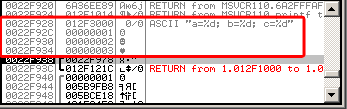
\includegraphics[width=0.5\textwidth]{patterns/03_printf/x86/olly3_stack.png}

\caption{\olly: stato dello stack dopo il push dei valori degli argomenti (il rettangolo rosso è stato aggiunto dall'autore per evidenziare la finestra)}
\end{figure}

Notiamo 3 colonne: indirizzo nello stack, valore nello stack ed alcuni commenti aggiuntivi di \olly.
\olly riconosce le stringhe \printf{}-like, e riporta quindi la stringa insieme ai 3 valori \emph{associati}.
% to be sync: \olly can detect pointers to ASCII strings in stack, so it reports the \printf{}-string here.

Facendo click destro sulla stringa di formato, quindi click su \q{Follow in dump},
è possibile vedere la format string nella finestra del debugger in basso a sinistra, che mostra una zona di memoria.
I valori mostrati possono anche essere modificati.
E' ad esempio possibile cambiare la format string, che renderebbe diverso il risultato dell'esempio.
Non è molto utile in questo particolare caso, ma può comunque essere un esercizio utile per iniziare a prendere dimestichezza con lo strumento.

\clearpage
Premiamo F8 (\stepover).

Il seguente output viene riportato in console:

\lstinputlisting{patterns/03_printf/x86/console.txt}

Vediamo come sono cambiati i registri e lo stack:

\begin{figure}[H]
\centering
\myincludegraphics{patterns/03_printf/x86/olly3_3.png}
\caption{\olly dopo dell'esecuzione di \printf{}}
\label{fig:printf3_olly_3}
\end{figure}

Il registro \EAX adesso contiene \GTT{0xD} (13).
Questo valore è corretto, poichè \printf restituisce il numero di caratteri stampati.
Il valore di \EIP è cambiato: adesso contiene infatti l'indirizzo dell'istruzione che viene dopo \INS{CALL printf}.
Anche i valori di \ECX e \EDX sono cambiati.
Apparentemente, i meccanismi interni alla funzione \printf hanno usato quei registri durante l'esecuzione di printf, per le sue necessità.

Un fatto molto importante è che nè il valore di ESP nè lo stack sono stati modificati!
Vediamo chiaramente che la format string ed i suoi 3 valori si trovano ancora lì.
Questo è infatti il comportamento della calling convention \emph{cdecl}: il \gls{callee} (la funzione chiamata) non ripristina
\ESP al suo valore precedente.
Farlo è una responsabilità del \gls{caller} (chiamante).

\clearpage
Premiamo F8 nuovamente per eseguire l'istruzione \INS{ADD ESP, 10}:

\begin{figure}[H]
\centering
\myincludegraphics{patterns/03_printf/x86/olly3_4.png}
\caption{\olly: dopo l'esecuzione dell'istruzione \INS{ADD ESP, 10}}
\label{fig:printf3_olly_4}
\end{figure}

\ESP è cambiato, ma i valori si trovano ancora sullo stack!
Ovviamente si: non c'è necessità di azzerare i valori o effettuare altre simili operazioni di "pulizia".
Qualunque cosa si trovi sopra lo stack pointer (\ac{SP})
è \emph{rumore} o \emph{\garbage{}} e non ha alcun significato.
Pulire i valori non utilizzati nello stack sarebbe una perdita di tempo inutile, e non vi è alcuna necessità di farlo.


\myparagraph{GCC}

Compiliamo lo stesso programma su Linux usando GCC 4.4.1, e diamo un'occhiata al risultato con \IDA:

\lstinputlisting[style=customasmx86]{patterns/03_printf/x86/x86_1.asm}

Si nota che la differenza tra il codice prodotto da MSVC e GCC risiede soltanto nel modo in cui gli argomenti sono memorizzati sullo stack.
In questo caso GCC lavora diversamente con lo stack, senza l'uso di \PUSH/\POP.

\myparagraph{GCC e GDB}
\myindex{GDB}

Proviamo l'esempio anche con \ac{GDB} su Linux.

L'opzione \GTT{-g} indica al compilatore di includere le informazioni di debug nel file eseguibile.

\begin{lstlisting}
$ gcc 1.c -g -o 1
\end{lstlisting}

\begin{lstlisting}
$ gdb 1
GNU gdb (GDB) 7.6.1-ubuntu
...
Reading symbols from /home/dennis/polygon/1...done.
\end{lstlisting}

\begin{lstlisting}[caption=impostiamo un breakpoint su \printf]
(gdb) b printf
Breakpoint 1 at 0x80482f0
\end{lstlisting}

Avviamolo.
Non abbiamo il sorgente della funzione \printf qui, quindi \ac{GDB} non può mostrarlo, anche se ne avrebbe la capacità.

\begin{lstlisting}
(gdb) run
Starting program: /home/dennis/polygon/1

Breakpoint 1, __printf (format=0x80484f0 "a=%d; b=%d; c=%d") at printf.c:29
29	printf.c: No such file or directory.
\end{lstlisting}

Stampiamo 10 elementi dello stack. La colonna più a sinistra contiene gli indirizzi nello stack.

\begin{lstlisting}
(gdb) x/10w $esp
0xbffff11c:	0x0804844a	0x080484f0	0x00000001	0x00000002
0xbffff12c:	0x00000003	0x08048460	0x00000000	0x00000000
0xbffff13c:	0xb7e29905	0x00000001
\end{lstlisting}

Il primo elemento è il \ac{RA} (\GTT{0x0804844a}).
Possiamo verificarlo disassemblando la memoria a questo indirizzo:

\begin{lstlisting}[label=NOP_as_XCHG_example,style=customasmx86]
(gdb) x/5i 0x0804844a
   0x804844a <main+45>:	mov    $0x0,%eax
   0x804844f <main+50>:	leave
   0x8048450 <main+51>:	ret
   0x8048451:	xchg   %ax,%ax
   0x8048453:	xchg   %ax,%ax
\end{lstlisting}

Le due istruzioni \INS{XCHG} sono istruzioni \q{inutili} (idle), analoghe a dei \ac{NOP}.

Il secondo elemento (\GTT{0x080484f0}) è l'indirizzo della format string:

\begin{lstlisting}
(gdb) x/s 0x080484f0
0x80484f0:	"a=%d; b=%d; c=%d"
\end{lstlisting}

I successivi 3 elementi (1, 2, 3) sono gli argomenti di \printf.
Il resto degli elementi potrebbe essere \q{immondizia} nello stack,
oppure valori provenienti da altre funzioni, come le loro variabili locali, etc.
Per il momento li possiamo ignorare.

Eseguiamo il comando \q{finish}.
Questo comando dice a GDB di \q{eseguire tutte le istruzioni fino alla fine della funzione}.
In questo caso: esegui fino alla fine di \printf.

\begin{lstlisting}
(gdb) finish
Run till exit from #0  __printf (format=0x80484f0 "a=%d; b=%d; c=%d") at printf.c:29
main () at 1.c:6
6		return 0;
Value returned is $2 = 13
\end{lstlisting}

\ac{GDB} mostra il risultato di \printf restituito in \EAX (13).
Questo è il numero di caratteri stampati, proprio come nell'esempio in \olly.

Vediamo anche \q{return 0;} e l'informazione che questa espressione si trova nel file \GTT{1.c} alla riga 6.
Infatti il file \GTT{1.c} si trova nella directory corrente, e \ac{GDB} trova la stringa lì.
Come fa \ac{GDB} a sapere quale riga del codice C viene eseguita?
Ciò è dovuto al fatto che il compilatore,
quando genera le informazioni di debug, salva anche una tabella di relazioni tra le righe del
codice sorgente e gli indirizzi delle istruzioni.
Dopotutto GDB è un \q{source-level debugger}.

Esaminiamo i registri.
13 in \EAX:

\begin{lstlisting}
(gdb) info registers
eax            0xd	13
ecx            0x0	0
edx            0x0	0
ebx            0xb7fc0000	-1208221696
esp            0xbffff120	0xbffff120
ebp            0xbffff138	0xbffff138
esi            0x0	0
edi            0x0	0
eip            0x804844a	0x804844a <main+45>
...
\end{lstlisting}

Disassembliamo le istruzioni correnti.
La freccia punta alla prossima istruzione da eseguire.

\begin{lstlisting}[style=customasmx86]
(gdb) disas
Dump of assembler code for function main:
   0x0804841d <+0>:	push   %ebp
   0x0804841e <+1>:	mov    %esp,%ebp
   0x08048420 <+3>:	and    $0xfffffff0,%esp
   0x08048423 <+6>:	sub    $0x10,%esp
   0x08048426 <+9>:	movl   $0x3,0xc(%esp)
   0x0804842e <+17>:	movl   $0x2,0x8(%esp)
   0x08048436 <+25>:	movl   $0x1,0x4(%esp)
   0x0804843e <+33>:	movl   $0x80484f0,(%esp)
   0x08048445 <+40>:	call   0x80482f0 <printf@plt>
=> 0x0804844a <+45>:	mov    $0x0,%eax
   0x0804844f <+50>:	leave
   0x08048450 <+51>:	ret
End of assembler dump.
\end{lstlisting}

\ac{GDB} usa la sintassi AT\&T di default.
Ma è anche possibile passare alla sintassi Intel:

\begin{lstlisting}[style=customasmx86]
(gdb) set disassembly-flavor intel
(gdb) disas
Dump of assembler code for function main:
   0x0804841d <+0>:	push   ebp
   0x0804841e <+1>:	mov    ebp,esp
   0x08048420 <+3>:	and    esp,0xfffffff0
   0x08048423 <+6>:	sub    esp,0x10
   0x08048426 <+9>:	mov    DWORD PTR [esp+0xc],0x3
   0x0804842e <+17>:	mov    DWORD PTR [esp+0x8],0x2
   0x08048436 <+25>:	mov    DWORD PTR [esp+0x4],0x1
   0x0804843e <+33>:	mov    DWORD PTR [esp],0x80484f0
   0x08048445 <+40>:	call   0x80482f0 <printf@plt>
=> 0x0804844a <+45>:	mov    eax,0x0
   0x0804844f <+50>:	leave
   0x08048450 <+51>:	ret
End of assembler dump.
\end{lstlisting}

Eseguiamo la prossima istruzione.
% to be sync: Execute next line of \CCpp{} code.
\ac{GDB} mostra la parentesi graffa chiusa, che sta a significare la fine del blocco di codice.

\begin{lstlisting}
(gdb) step
7	};
\end{lstlisting}

Esaminiamo i registri dopo l'esecuzione dell'istruzione \INS{MOV EAX, 0}.
\EAX è zero a questo punto.

\begin{lstlisting}
(gdb) info registers
eax            0x0	0
ecx            0x0	0
edx            0x0	0
ebx            0xb7fc0000	-1208221696
esp            0xbffff120	0xbffff120
ebp            0xbffff138	0xbffff138
esi            0x0	0
edi            0x0	0
eip            0x804844f	0x804844f <main+50>
...
\end{lstlisting}
